% Options for packages loaded elsewhere
\PassOptionsToPackage{unicode}{hyperref}
\PassOptionsToPackage{hyphens}{url}
%
\documentclass[
  ignorenonframetext,
]{beamer}
\usepackage{pgfpages}
\setbeamertemplate{caption}[numbered]
\setbeamertemplate{caption label separator}{: }
\setbeamercolor{caption name}{fg=normal text.fg}
\beamertemplatenavigationsymbolsempty
% Prevent slide breaks in the middle of a paragraph
\widowpenalties 1 10000
\raggedbottom
\setbeamertemplate{part page}{
  \centering
  \begin{beamercolorbox}[sep=16pt,center]{part title}
    \usebeamerfont{part title}\insertpart\par
  \end{beamercolorbox}
}
\setbeamertemplate{section page}{
  \centering
  \begin{beamercolorbox}[sep=12pt,center]{part title}
    \usebeamerfont{section title}\insertsection\par
  \end{beamercolorbox}
}
\setbeamertemplate{subsection page}{
  \centering
  \begin{beamercolorbox}[sep=8pt,center]{part title}
    \usebeamerfont{subsection title}\insertsubsection\par
  \end{beamercolorbox}
}
\AtBeginPart{
  \frame{\partpage}
}
\AtBeginSection{
  \ifbibliography
  \else
    \frame{\sectionpage}
  \fi
}
\AtBeginSubsection{
  \frame{\subsectionpage}
}
\usepackage{amsmath,amssymb}
\usepackage{iftex}
\ifPDFTeX
  \usepackage[T1]{fontenc}
  \usepackage[utf8]{inputenc}
  \usepackage{textcomp} % provide euro and other symbols
\else % if luatex or xetex
  \usepackage{unicode-math} % this also loads fontspec
  \defaultfontfeatures{Scale=MatchLowercase}
  \defaultfontfeatures[\rmfamily]{Ligatures=TeX,Scale=1}
\fi
\usepackage{lmodern}
\usetheme[]{Boadilla}
\ifPDFTeX\else
  % xetex/luatex font selection
\fi
% Use upquote if available, for straight quotes in verbatim environments
\IfFileExists{upquote.sty}{\usepackage{upquote}}{}
\IfFileExists{microtype.sty}{% use microtype if available
  \usepackage[]{microtype}
  \UseMicrotypeSet[protrusion]{basicmath} % disable protrusion for tt fonts
}{}
\makeatletter
\@ifundefined{KOMAClassName}{% if non-KOMA class
  \IfFileExists{parskip.sty}{%
    \usepackage{parskip}
  }{% else
    \setlength{\parindent}{0pt}
    \setlength{\parskip}{6pt plus 2pt minus 1pt}}
}{% if KOMA class
  \KOMAoptions{parskip=half}}
\makeatother
\usepackage{xcolor}
\newif\ifbibliography
\usepackage{color}
\usepackage{fancyvrb}
\newcommand{\VerbBar}{|}
\newcommand{\VERB}{\Verb[commandchars=\\\{\}]}
\DefineVerbatimEnvironment{Highlighting}{Verbatim}{commandchars=\\\{\}}
% Add ',fontsize=\small' for more characters per line
\usepackage{framed}
\definecolor{shadecolor}{RGB}{248,248,248}
\newenvironment{Shaded}{\begin{snugshade}}{\end{snugshade}}
\newcommand{\AlertTok}[1]{\textcolor[rgb]{0.94,0.16,0.16}{#1}}
\newcommand{\AnnotationTok}[1]{\textcolor[rgb]{0.56,0.35,0.01}{\textbf{\textit{#1}}}}
\newcommand{\AttributeTok}[1]{\textcolor[rgb]{0.13,0.29,0.53}{#1}}
\newcommand{\BaseNTok}[1]{\textcolor[rgb]{0.00,0.00,0.81}{#1}}
\newcommand{\BuiltInTok}[1]{#1}
\newcommand{\CharTok}[1]{\textcolor[rgb]{0.31,0.60,0.02}{#1}}
\newcommand{\CommentTok}[1]{\textcolor[rgb]{0.56,0.35,0.01}{\textit{#1}}}
\newcommand{\CommentVarTok}[1]{\textcolor[rgb]{0.56,0.35,0.01}{\textbf{\textit{#1}}}}
\newcommand{\ConstantTok}[1]{\textcolor[rgb]{0.56,0.35,0.01}{#1}}
\newcommand{\ControlFlowTok}[1]{\textcolor[rgb]{0.13,0.29,0.53}{\textbf{#1}}}
\newcommand{\DataTypeTok}[1]{\textcolor[rgb]{0.13,0.29,0.53}{#1}}
\newcommand{\DecValTok}[1]{\textcolor[rgb]{0.00,0.00,0.81}{#1}}
\newcommand{\DocumentationTok}[1]{\textcolor[rgb]{0.56,0.35,0.01}{\textbf{\textit{#1}}}}
\newcommand{\ErrorTok}[1]{\textcolor[rgb]{0.64,0.00,0.00}{\textbf{#1}}}
\newcommand{\ExtensionTok}[1]{#1}
\newcommand{\FloatTok}[1]{\textcolor[rgb]{0.00,0.00,0.81}{#1}}
\newcommand{\FunctionTok}[1]{\textcolor[rgb]{0.13,0.29,0.53}{\textbf{#1}}}
\newcommand{\ImportTok}[1]{#1}
\newcommand{\InformationTok}[1]{\textcolor[rgb]{0.56,0.35,0.01}{\textbf{\textit{#1}}}}
\newcommand{\KeywordTok}[1]{\textcolor[rgb]{0.13,0.29,0.53}{\textbf{#1}}}
\newcommand{\NormalTok}[1]{#1}
\newcommand{\OperatorTok}[1]{\textcolor[rgb]{0.81,0.36,0.00}{\textbf{#1}}}
\newcommand{\OtherTok}[1]{\textcolor[rgb]{0.56,0.35,0.01}{#1}}
\newcommand{\PreprocessorTok}[1]{\textcolor[rgb]{0.56,0.35,0.01}{\textit{#1}}}
\newcommand{\RegionMarkerTok}[1]{#1}
\newcommand{\SpecialCharTok}[1]{\textcolor[rgb]{0.81,0.36,0.00}{\textbf{#1}}}
\newcommand{\SpecialStringTok}[1]{\textcolor[rgb]{0.31,0.60,0.02}{#1}}
\newcommand{\StringTok}[1]{\textcolor[rgb]{0.31,0.60,0.02}{#1}}
\newcommand{\VariableTok}[1]{\textcolor[rgb]{0.00,0.00,0.00}{#1}}
\newcommand{\VerbatimStringTok}[1]{\textcolor[rgb]{0.31,0.60,0.02}{#1}}
\newcommand{\WarningTok}[1]{\textcolor[rgb]{0.56,0.35,0.01}{\textbf{\textit{#1}}}}
\usepackage{longtable,booktabs,array}
\usepackage{calc} % for calculating minipage widths
\usepackage{caption}
% Make caption package work with longtable
\makeatletter
\def\fnum@table{\tablename~\thetable}
\makeatother
\usepackage{graphicx}
\makeatletter
\def\maxwidth{\ifdim\Gin@nat@width>\linewidth\linewidth\else\Gin@nat@width\fi}
\def\maxheight{\ifdim\Gin@nat@height>\textheight\textheight\else\Gin@nat@height\fi}
\makeatother
% Scale images if necessary, so that they will not overflow the page
% margins by default, and it is still possible to overwrite the defaults
% using explicit options in \includegraphics[width, height, ...]{}
\setkeys{Gin}{width=\maxwidth,height=\maxheight,keepaspectratio}
% Set default figure placement to htbp
\makeatletter
\def\fps@figure{htbp}
\makeatother
\setlength{\emergencystretch}{3em} % prevent overfull lines
\providecommand{\tightlist}{%
  \setlength{\itemsep}{0pt}\setlength{\parskip}{0pt}}
\setcounter{secnumdepth}{-\maxdimen} % remove section numbering
\usepackage{graphicx}
\logo{\ifnum\thepage>1\hfill
\includegraphics[width=1cm]{logo}\fi}
\titlegraphic{
\includegraphics[width=3cm]{logo}}
\ifLuaTeX
  \usepackage{selnolig}  % disable illegal ligatures
\fi
\usepackage{bookmark}
\IfFileExists{xurl.sty}{\usepackage{xurl}}{} % add URL line breaks if available
\urlstyle{same}
\hypersetup{
  pdftitle={Descriptive Statistics},
  pdfauthor={Pablo E. Gutierrez-Fonseca},
  hidelinks,
  pdfcreator={LaTeX via pandoc}}

\title{Descriptive Statistics}
\author{Pablo E. Gutierrez-Fonseca}
\date{Fall 2024}

\begin{document}
\frame{\titlepage}

\begin{frame}{Why describe data?}
\phantomsection\label{why-describe-data}
\begin{itemize}
\tightlist
\item
  Determine if our sample reflects the population of interest.
\end{itemize}

\begin{itemize}
\tightlist
\item
  Identify outliers.
\end{itemize}

\begin{itemize}
\tightlist
\item
  Obtain metrics necessary for inferential tests.
\end{itemize}

\begin{itemize}
\tightlist
\item
  Understand the distribution of our data values (i.e., test for
  normality).
\end{itemize}

\begin{itemize}
\tightlist
\item
  Identify the type of statistical test to run.
\end{itemize}
\end{frame}

\begin{frame}{Data description and visualization}
\phantomsection\label{data-description-and-visualization}
\begin{itemize}
\tightlist
\item
  We can examine our data and run statistical tests to see if the
  distribution approximates a normal curve.\\
\item
  Typically, we start by visualizing our data.
\end{itemize}

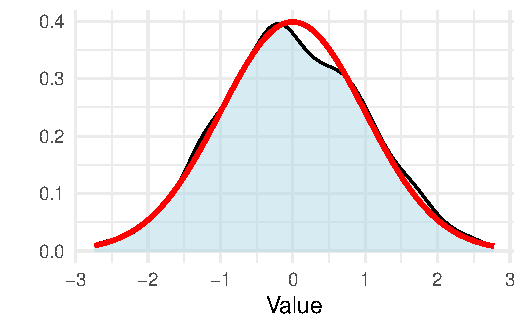
\includegraphics{M4-Descriptice-Statistics_files/figure-beamer/unnamed-chunk-1-1.pdf}
\end{frame}

\begin{frame}{Histogram basic}
\phantomsection\label{histogram-basic}
\begin{itemize}
\tightlist
\item
  Continuous data are most commonly visualized using Histograms.
\end{itemize}

\begin{figure}
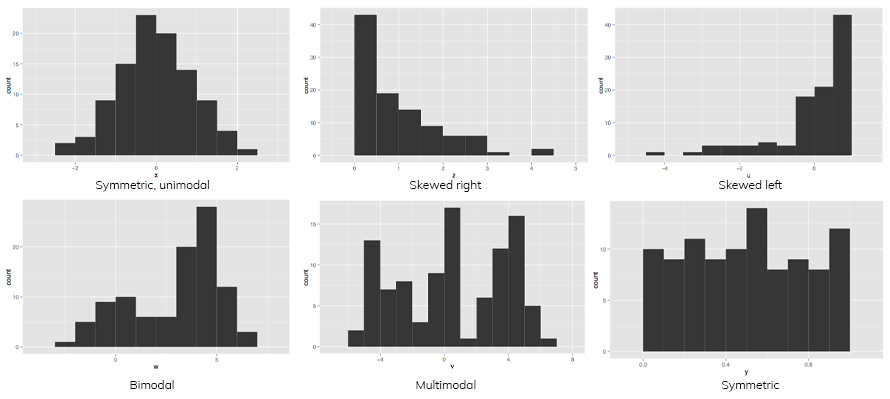
\includegraphics[width=0.8\linewidth]{fig/Histogram} \end{figure}
\end{frame}

\begin{frame}{Box and Whisker Basics}
\phantomsection\label{box-and-whisker-basics}
\begin{figure}
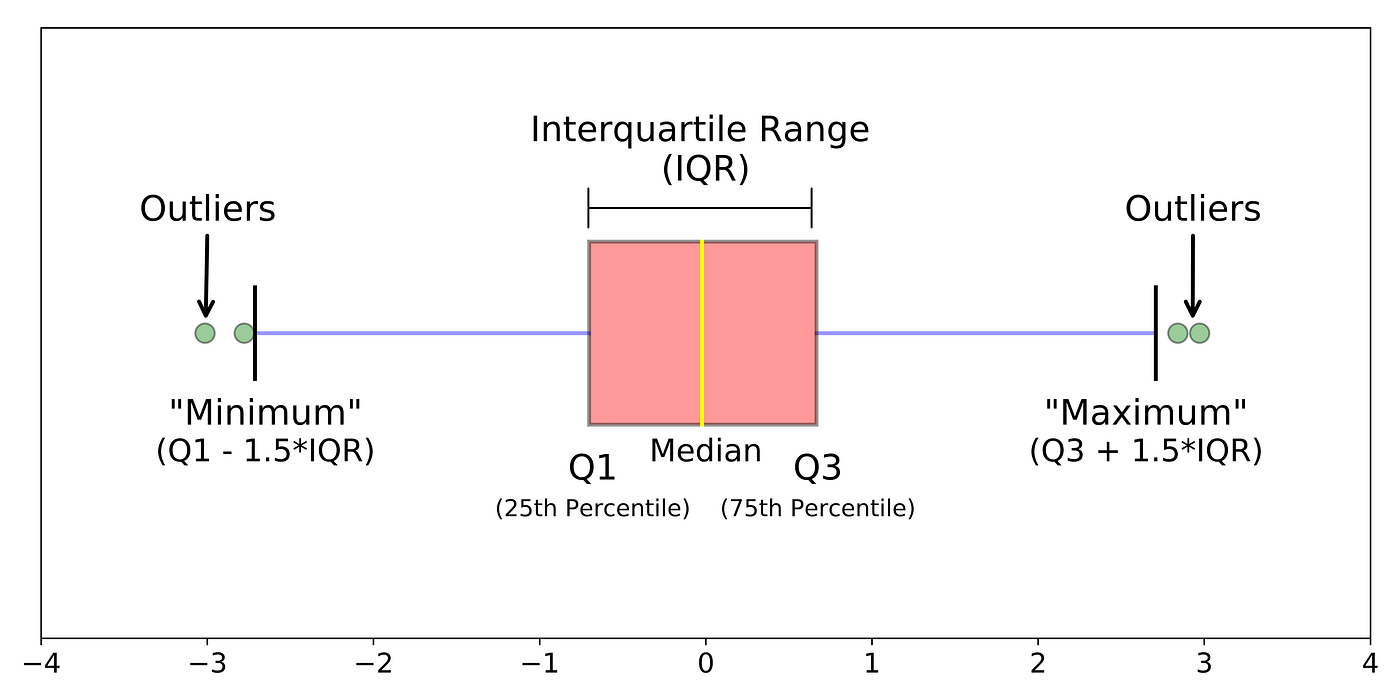
\includegraphics[width=0.8\linewidth]{fig/box} \end{figure}
\end{frame}

\begin{frame}{Metrics to Describe data distribution.}
\phantomsection\label{metrics-to-describe-data-distribution.}
\begin{itemize}
\item
  Data and their associated distributions can be described in four
  primary way:

  \begin{itemize}
  \tightlist
  \item
    Central Tendency (mean, median, mode)
  \item
    Variability (standard deviation, variance, quantiles)
  \item
    Skew
  \item
    Kurtosis (Peakedness)
  \end{itemize}
\end{itemize}
\end{frame}

\begin{frame}{Metrics to Describe data distribution.}
\phantomsection\label{metrics-to-describe-data-distribution.-1}
\begin{itemize}
\item
  Data and their associated distributions can be described in four
  primary way:

  \begin{itemize}
  \tightlist
  \item
    \textbf{Central Tendency (mean, median, mode)}
  \item
    Variability (standard deviation, variance, quantiles)
  \item
    Skew
  \item
    Kurtosis (Peakedness)
  \end{itemize}
\end{itemize}
\end{frame}

\begin{frame}{Central tendency}
\phantomsection\label{central-tendency}
\begin{itemize}
\tightlist
\item
  Mean (Sum of scores/N)

  \begin{itemize}
  \tightlist
  \item
    Most often used measure of central tendency.
  \item
    Works well with normal and relatively normal curves.
  \end{itemize}
\item
  Median (50th Percentile)

  \begin{itemize}
  \tightlist
  \item
    No formula. Rank order observations then find the middle.
  \item
    The second most used measure of central tendency.
  \item
    Works best with highly skewed populations.
  \end{itemize}
\item
  Mode (Most Frequent Score)

  \begin{itemize}
  \tightlist
  \item
    Least used measure of central tendency.
  \item
    Works best for highly irregular and multimodal distributions.
  \end{itemize}
\end{itemize}
\end{frame}

\begin{frame}{Central tendency: Mean}
\phantomsection\label{central-tendency-mean}
\begin{itemize}
\item
  Sample mean is the measure of central tendency that best represents
  the population mean.
\item
  Mean is \textbf{very} sensitive to extreme scores that can ``skew'' or
  distort findings.
\end{itemize}
\end{frame}

\begin{frame}{Central tendency: Median}
\phantomsection\label{central-tendency-median}
\begin{itemize}
\tightlist
\item
  Percentiles are used to define the percent of cases equal to and below
  a certain point on a distribution.

  \begin{itemize}
  \tightlist
  \item
    The median \textbf{is the 50th percentile } half of all observations
    fall at or below this value.
  \end{itemize}
\end{itemize}

\begin{itemize}
\tightlist
\item
  But lots of other percentiles are also important.
\end{itemize}
\end{frame}

\begin{frame}{A little about Percentiles}
\phantomsection\label{a-little-about-percentiles}
\begin{itemize}
\tightlist
\item
  Quartiles are a common percentile used to represent the value below
  which.

  \begin{itemize}
  \tightlist
  \item
    25\% (Q1 or first quartile)\\
  \item
    75\% (Q3 or third quartile)
  \end{itemize}
\end{itemize}

\begin{figure}
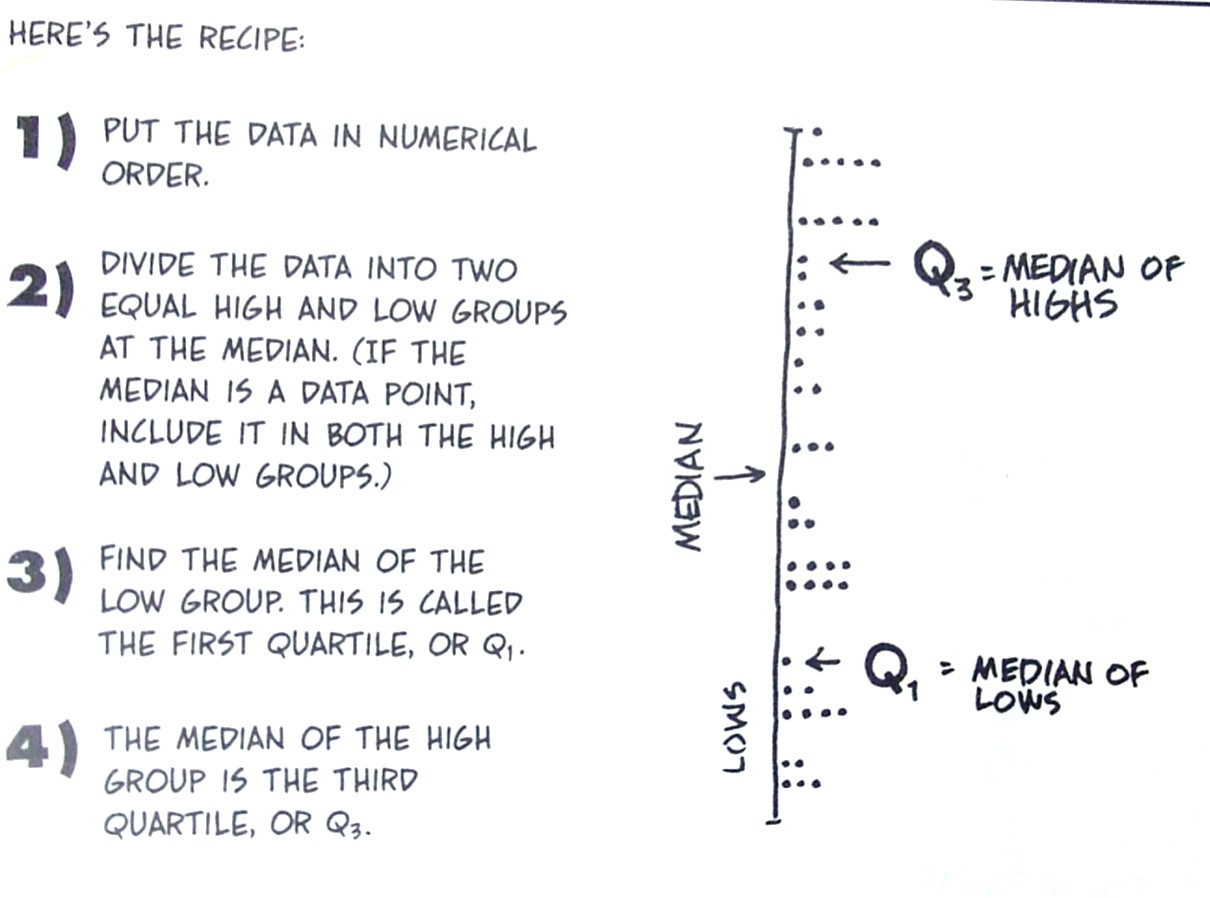
\includegraphics[width=0.4\linewidth]{fig/quartiles} \end{figure}
\end{frame}

\begin{frame}{When to use What}
\phantomsection\label{when-to-use-what}
\begin{itemize}
\tightlist
\item
  Use the \textbf{Mode} when the data are categorical:

  \begin{itemize}
  \tightlist
  \item
    \textbf{Mode}: is the value that occurs most frequently in your
    data.\\
  \item
    This is because having the same value occur for measurements with
    many significant digits is highly unlikely.
  \end{itemize}
\end{itemize}

\begin{itemize}
\tightlist
\item
  Use the \textbf{Median} when you have extreme scores:

  \begin{itemize}
  \tightlist
  \item
    \textbf{Median}: is simply the value that falls in the middle of all
    your data.
  \end{itemize}
\end{itemize}

\begin{itemize}
\tightlist
\item
  Use the \textbf{Mean} the rest of the time.
\end{itemize}

\begin{figure}
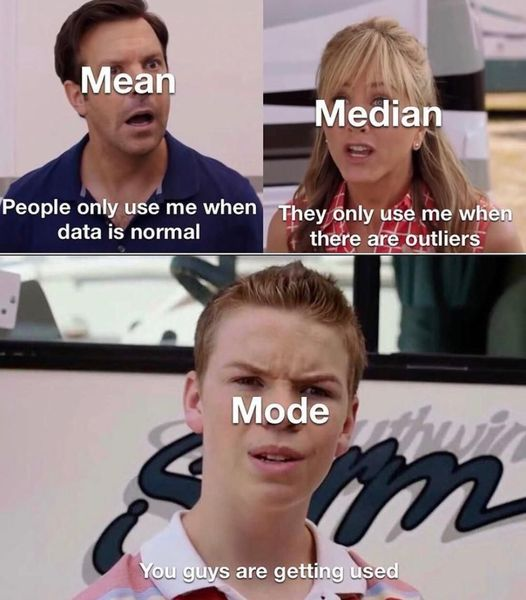
\includegraphics[width=0.25\linewidth]{fig/CnetralTendency} \end{figure}
\end{frame}

\begin{frame}{Metrics to Describe data distribution.}
\phantomsection\label{metrics-to-describe-data-distribution.-2}
\begin{itemize}
\item
  Data and their associated distributions can be described in four
  primary way:

  \begin{itemize}
  \tightlist
  \item
    Central Tendency (mean, median, mode)
  \item
    \textbf{Variability (standard deviation, variance, quantiles)}
  \item
    Skew
  \item
    Kurtosis (Peakedness)
  \end{itemize}
\end{itemize}
\end{frame}

\begin{frame}{Variability}
\phantomsection\label{variability}
\begin{figure}
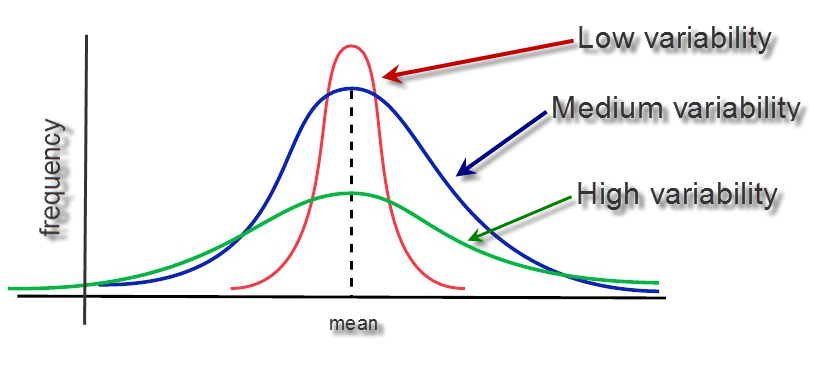
\includegraphics[width=0.8\linewidth]{fig/variability} \end{figure}
\end{frame}

\begin{frame}{Variability: Standard Deviation}
\phantomsection\label{variability-standard-deviation}
\begin{itemize}
\tightlist
\item
  Standard Deviation measures how spread out the numbers in a dataset
  are around the mean.
\end{itemize}

\begin{itemize}
\tightlist
\item
  The sample standard deviation \(s\) is calculated as:
  \[s = \sqrt{\frac{\sum_{i=1}^{n} (x_i - \bar{x})^2}{n - 1}}\]
\end{itemize}
\end{frame}

\begin{frame}{Variability}
\phantomsection\label{variability-1}
\begin{itemize}
\tightlist
\item
  \textbf{Variance} measures the average of the squared differences from
  the mean, indicating how spread out the data points are.
\end{itemize}

\begin{itemize}
\tightlist
\item
  The variance \(\sigma^2\) is calculated as:
  \[s^2 = \frac{\sum_{i=1}^{n} (x_i - \bar{x})^2}{n - 1}\]
\end{itemize}
\end{frame}

\begin{frame}{Variability: Range}
\phantomsection\label{variability-range}
\begin{itemize}
\tightlist
\item
  \textbf{Range} is the difference between the largest and smallest
  values in a dataset, providing a measure of the spread or dispersion
  of the data.
\end{itemize}

\begin{itemize}
\tightlist
\item
  The range is calculated as:
  \[\text{Range} = \text{max}(x) - \text{min}(x)\]
\end{itemize}
\end{frame}

\begin{frame}{Percentiles are useful for spread too}
\phantomsection\label{percentiles-are-useful-for-spread-too}
\begin{itemize}
\item
  You can use percentiles to get a feel for how spread out the data is
  and where most of your observations are contained:

  \begin{itemize}
  \tightlist
  \item
    Inter-quartile range (IQR) = Q3 - Q1
  \end{itemize}
\end{itemize}

\begin{figure}
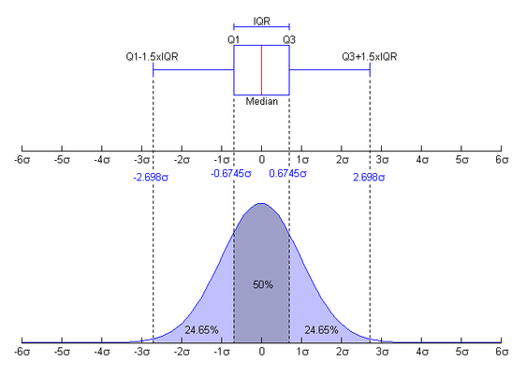
\includegraphics[width=0.6\linewidth]{fig/iqr} \end{figure}
\end{frame}

\begin{frame}{Identifying outliers}
\phantomsection\label{identifying-outliers}
\begin{itemize}
\tightlist
\item
  An outlier is an observation that lies outside the overall pattern of
  a distribution (Moore and McCabe 1999).
\end{itemize}

\begin{itemize}
\tightlist
\item
  Usually, the presence of an outlier indicates some sort of problem.
  (e.g.~an error in measurement or sample selection).
\end{itemize}

\begin{itemize}
\tightlist
\item
  But they may also be an indicator of novel data or identification of
  unique and exciting observations.
\end{itemize}
\end{frame}

\begin{frame}{Identifying outliers}
\phantomsection\label{identifying-outliers-1}
\begin{itemize}
\tightlist
\item
  The first and third quantiles (Q1 and Q3) are often calculated to
  identify outliers.
\end{itemize}

\begin{itemize}
\tightlist
\item
  One method for systematically identifying outliers uses:

  \begin{itemize}
  \tightlist
  \item
    Q1 - (1.5 * the inter-quartile range)
  \item
    Q3 + (1.5 * the inter-quartile range)
  \end{itemize}
\end{itemize}

\begin{itemize}
\tightlist
\item
  Others identify outliers as any values below the 0.5th or above the
  99.5th percentile.
\end{itemize}
\end{frame}

\begin{frame}{When to use What}
\phantomsection\label{when-to-use-what-1}
\begin{itemize}
\tightlist
\item
  Use the \textbf{Standard deviation (SD)} in most cases.

  \begin{itemize}
  \tightlist
  \item
    SD quantifies how far, on average, each observation is from the
    mean.
  \item
    The larger the SD, the more highly variable your data.
  \end{itemize}
\end{itemize}

\begin{itemize}
\tightlist
\item
  Use \textbf{range (R)} when describing predictive models.

  \begin{itemize}
  \tightlist
  \item
    R is simply the maximum minus the minimum value in your data set
  \item
    R is important when modeling or making predictions, since your
    algorithms are valid only over the range of values used to calibrate
    your predictive model
  \end{itemize}
\end{itemize}

\begin{itemize}
\tightlist
\item
  Use the \textbf{IQR} to identify and test potential outliers in your
  data.
\end{itemize}
\end{frame}

\begin{frame}{Metrics to Describe data distribution.}
\phantomsection\label{metrics-to-describe-data-distribution.-3}
\begin{itemize}
\item
  Data and their associated distributions can be described in four
  primary way:

  \begin{itemize}
  \tightlist
  \item
    Central Tendency (mean, median, mode)
  \item
    Variability (standard deviation, variance, quantiles)
  \item
    \textbf{Skew}
  \item
    Kurtosis (Peakedness)
  \end{itemize}
\end{itemize}
\end{frame}

\begin{frame}{Skewness}
\phantomsection\label{skewness}
\begin{itemize}
\tightlist
\item
  Skewness: This metric quantifies how balanced (symmetrical) your
  distribution curve is.
\end{itemize}

\begin{figure}
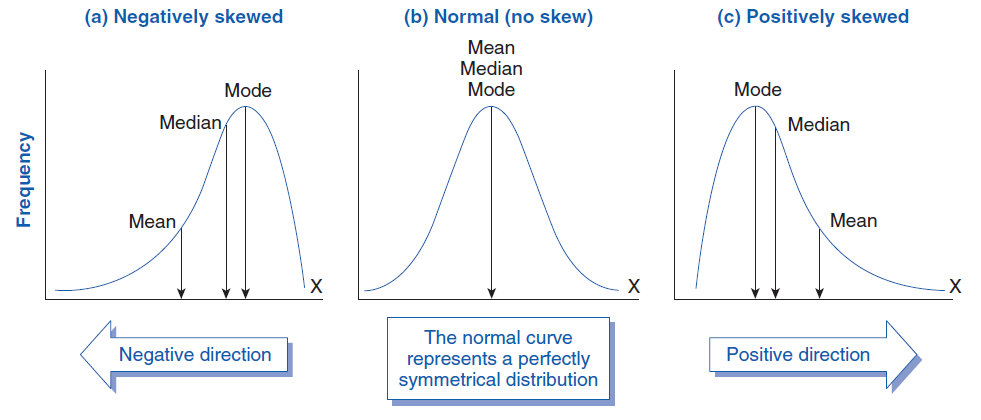
\includegraphics[width=0.8\linewidth]{fig/skewness} \end{figure}
\end{frame}

\begin{frame}{Skewness}
\phantomsection\label{skewness-1}
\begin{itemize}
\tightlist
\item
  A normal distribution will have its mean and median values located
  somewhere near the center of its range.
\end{itemize}

\begin{figure}
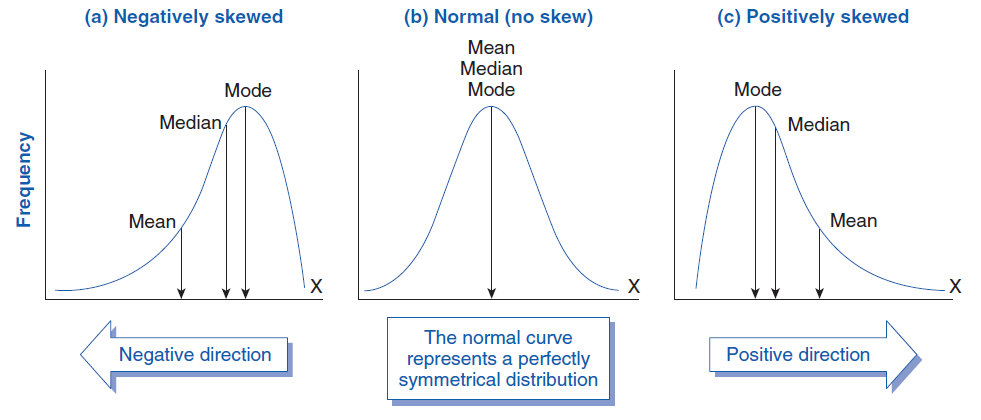
\includegraphics[width=0.8\linewidth]{fig/skewness} \end{figure}
\end{frame}

\begin{frame}{Skewness}
\phantomsection\label{skewness-2}
\begin{itemize}
\tightlist
\item
  Skew of this peak away from center is common when extreme values pull
  the median away from the mean.

  \begin{figure}
  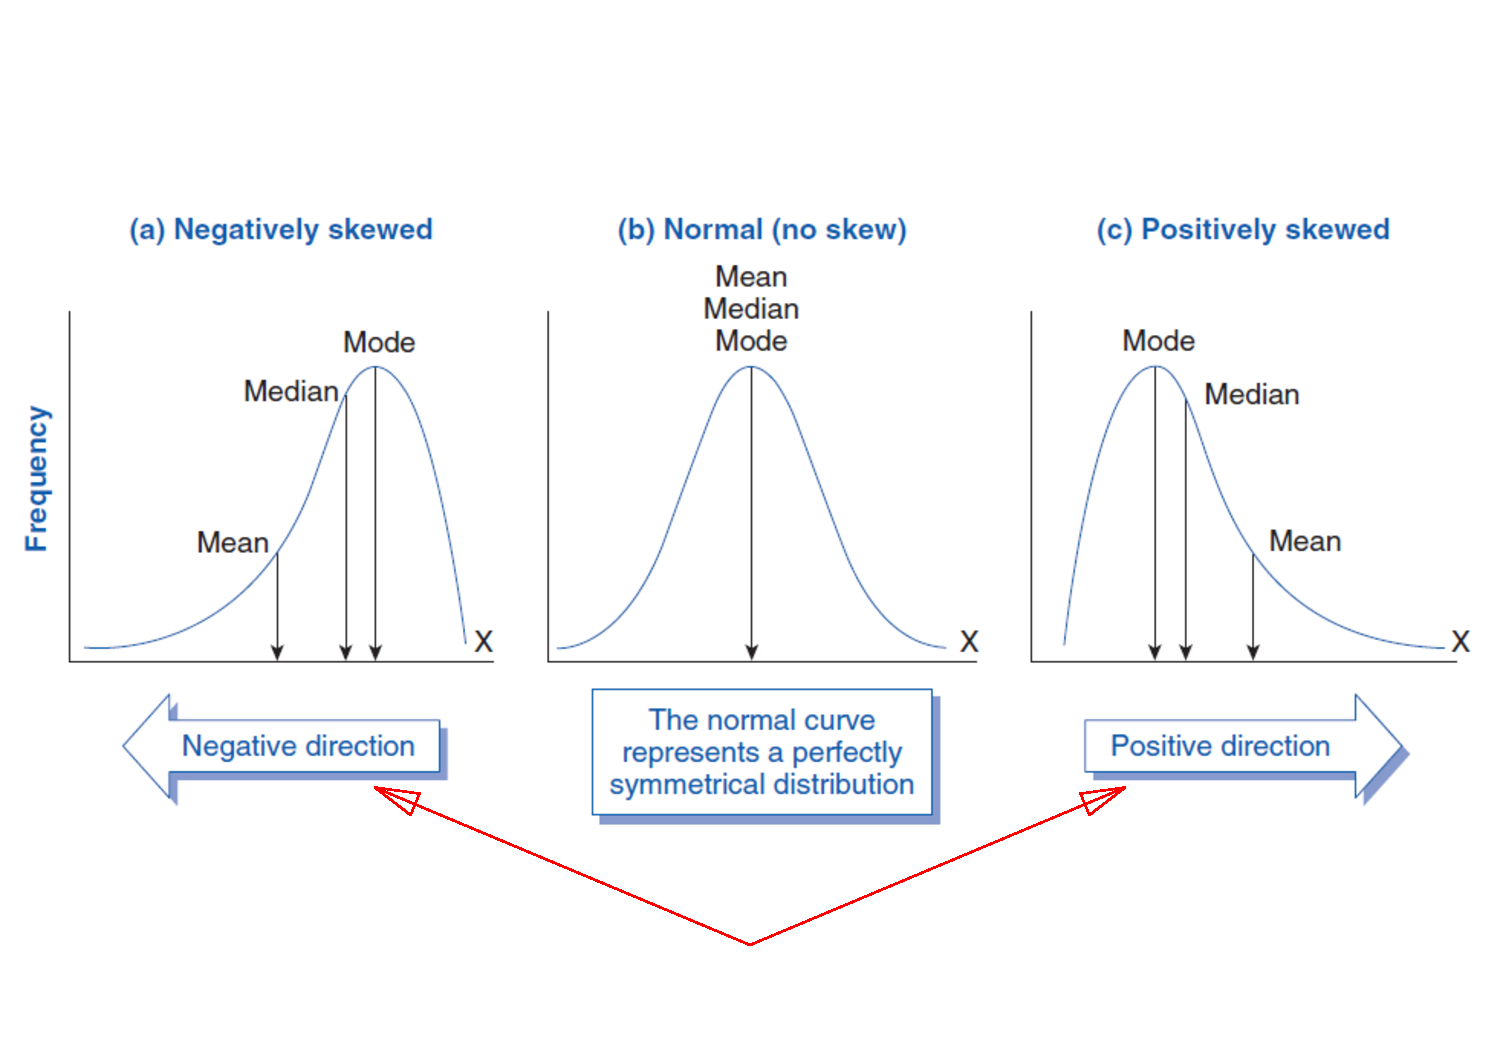
\includegraphics[width=0.8\linewidth]{M4-Descriptice-Statistics_files/figure-beamer/unnamed-chunk-13-1} \end{figure}
\end{itemize}
\end{frame}

\begin{frame}{Skewness}
\phantomsection\label{skewness-3}
\begin{itemize}
\tightlist
\item
  \textbf{Positive Skew}: the ``slide'' takes you in a positive
  direction.

  \begin{itemize}
  \tightlist
  \item
    The mean is bigger than the median (which is why the slide is being
    pulled to higher values).
  \end{itemize}
\end{itemize}

\begin{itemize}
\tightlist
\item
  \textbf{Negative Skew}: the ``slide'' takes you in a negative
  direction.

  \begin{itemize}
  \tightlist
  \item
    The mean is smaller than the median (which is why the slide is being
    pulled to lower values).
  \end{itemize}
\end{itemize}

\begin{figure}
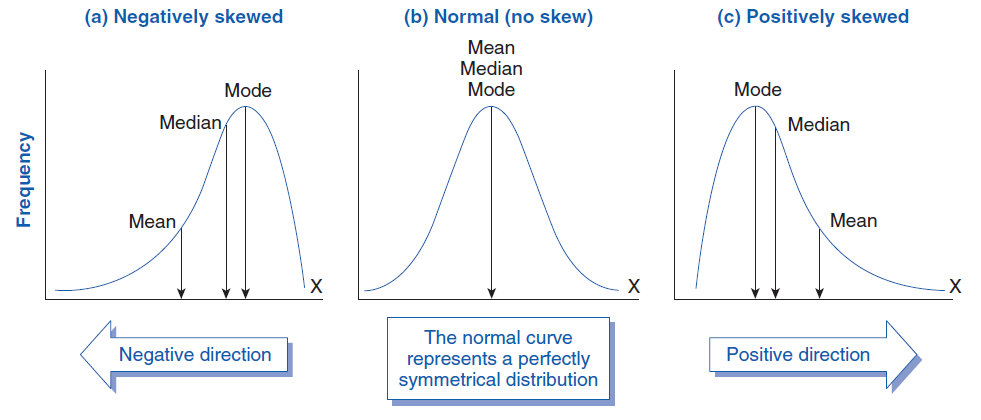
\includegraphics[width=0.8\linewidth]{fig/skewness} \end{figure}
\end{frame}

\begin{frame}{Calculating Skew}
\phantomsection\label{calculating-skew}
\begin{itemize}
\tightlist
\item
  Negative value = Negative Skew.
\end{itemize}

\begin{itemize}
\tightlist
\item
  Positive value = Positive Skew
\end{itemize}

\begin{itemize}
\tightlist
\item
  Positive value = Normal distribution
\end{itemize}

\[\text{Skewness} = \frac{3(\bar{x} - \text{Median})}{\text{SD}}\]
\end{frame}

\begin{frame}{Skewness: Significant?}
\phantomsection\label{skewness-significant}
\begin{itemize}
\item
  To determine if this deviation from zero in the skew statistic is
  likely a significant departure from normality, compare it to the
  \textbf{standard error of skew (ses)}.
\item
  If the skew you have calculated is more than \textbf{2 times the ses},
  then you likely have significant skew, which means you have
  \textbf{non normal data} and should consider a nonparametric test for
  your statistical analyses
\end{itemize}

\[
\begin{array}{cc}
ses = \sqrt{\frac{6}{n}} & \hspace{1cm} \text{Skewness} = \frac{3(\bar{x} - \text{Median})}{\text{SD}}
\end{array}
\]
\end{frame}

\begin{frame}{Metrics to Describe data distribution.}
\phantomsection\label{metrics-to-describe-data-distribution.-4}
\begin{itemize}
\item
  Data and their associated distributions can be described in four
  primary way:

  \begin{itemize}
  \tightlist
  \item
    Central Tendency (mean, median, mode)
  \item
    Variability (standard deviation, variance, quantiles)
  \item
    Skew
  \item
    \textbf{Kurtosis (Peakedness)}
  \end{itemize}
\end{itemize}
\end{frame}

\begin{frame}{Kurtosis}
\phantomsection\label{kurtosis}
\begin{itemize}
\tightlist
\item
  \textbf{Kurtosis} is simply a measure of how pointy or flat the peak
  of your distribution curve is.
\end{itemize}

\begin{itemize}
\tightlist
\item
  Any deviation from a bell shape, with the peak either too flat
  (platykurtic) or too peaked (leptokurtic), suggests that your data are
  not normally distributed.
\end{itemize}

\begin{figure}
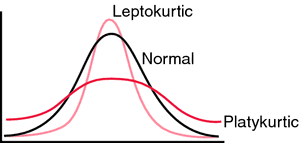
\includegraphics[width=0.6\linewidth]{fig/kurtosis} \end{figure}
\end{frame}

\begin{frame}{Kurtosis}
\phantomsection\label{kurtosis-1}
\begin{itemize}
\tightlist
\item
  Positive values = Leptokurtic.
\end{itemize}

\begin{itemize}
\tightlist
\item
  Zero = Mesokurtic = normal (bell-shaped).
\end{itemize}

\begin{itemize}
\tightlist
\item
  Negative values = Platykurtic.
\end{itemize}

\[
\text{Kurtosis} = \frac{\sum(\left( \frac{x_i - \bar{x}}{\text{SD}} \right)^4 - 3)}{n}
\]
\end{frame}

\begin{frame}{Kurtosis: Significant?}
\phantomsection\label{kurtosis-significant}
\begin{itemize}
\item
  To determine if this deviation from zero in the kurtosis statistic is
  likely a significant departure from normality, compare it to the
  \textbf{standard error of kurtosis (sek)}.
\item
  If the kurtosis you have calculated is more than \textbf{twice the
  sek}, you likely have \textbf{non normal data} and should consider a
  nonparametric test for your statistical analyses.
\end{itemize}

\[
\begin{array}{cc}
sek = \sqrt{\frac{24}{n}} & \hspace{2cm} \text{Kurtosis} = \frac{\sum \left( \frac{x_i - \bar{x}}{\text{SD}} \right)^4 - 3}{n}
\end{array}
\]
\end{frame}

\begin{frame}{Some Visual Examples}
\phantomsection\label{some-visual-examples}
\begin{itemize}
\item
  How can climate change?
\item
  Change in \textbf{central tendency}.
\end{itemize}

\begin{figure}
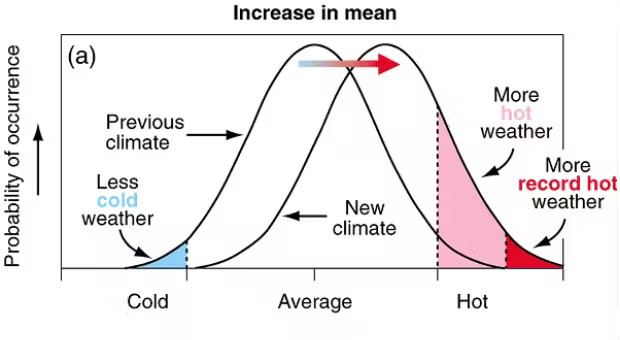
\includegraphics[width=0.6\linewidth]{fig/climate1} \end{figure}
\end{frame}

\begin{frame}{Some Visual Examples}
\phantomsection\label{some-visual-examples-1}
\begin{itemize}
\tightlist
\item
  How can climate change?
\end{itemize}

\begin{itemize}
\tightlist
\item
  Change in \textbf{spread and shape}.
\end{itemize}

\begin{figure}
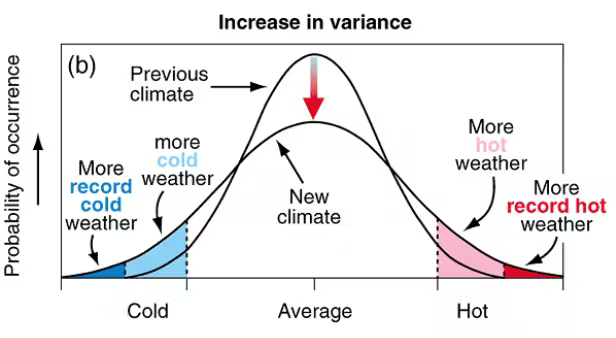
\includegraphics[width=0.6\linewidth]{fig/climate2} \end{figure}
\end{frame}

\begin{frame}{Some Visual Examples}
\phantomsection\label{some-visual-examples-2}
\begin{itemize}
\tightlist
\item
  How can climate change?
\end{itemize}

\begin{itemize}
\tightlist
\item
  Change in \textbf{both}.
\end{itemize}

\begin{figure}
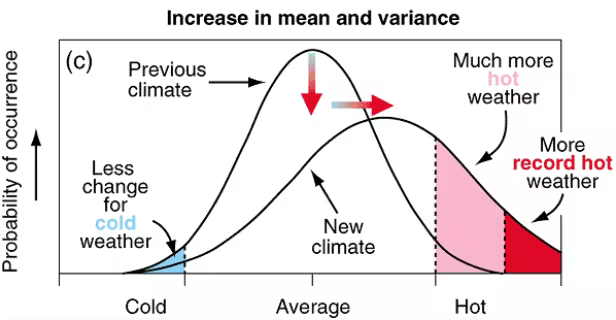
\includegraphics[width=0.6\linewidth]{fig/climate3} \end{figure}
\end{frame}

\begin{frame}{Data Distributions}
\phantomsection\label{data-distributions}
\end{frame}

\begin{frame}{Data Distributions}
\phantomsection\label{data-distributions-1}
\begin{itemize}
\item
  There are various types of data distributions, each with its own
  unique properties and implications.
\item
  In nature, most data are normally distributed.
\item
  The central limit theorem (CLT) states that the distribution of sample
  means approximates a normal distribution as the sample size gets
  larger, regardless of the population's distribution.
\end{itemize}

\[
\bar{X}_n \sim N\left(\mu, \frac{\sigma^2}{n}\right)
\] - \(\bar{X}_n\): The sample mean of size \(n\).\\
- \(N(\mu, \frac{\sigma^2}{n})\): The normal distribution with mean
\(\mu\) (the population mean) and variance \(\frac{\sigma^2}{n}\), where
\(\sigma^2\) is the population variance and \(n\) is the sample size.
\end{frame}

\begin{frame}{Why do we care if our data is normal?}
\phantomsection\label{why-do-we-care-if-our-data-is-normal}
\begin{itemize}
\tightlist
\item
  The math ``under the hood'' of many analyses \textbf{expects that data
  is normally distributed} - if it isn't, you'll still get an answer,
  but it won't actually be saying what you think it is saying.
\end{itemize}
\end{frame}

\begin{frame}{Why do we care about \textbf{skew} and \textbf{kurtosis}?}
\phantomsection\label{why-do-we-care-about-skew-and-kurtosis}
\begin{itemize}
\tightlist
\item
  Because many statistical analyses assume a normal distribution of the
  data, testing for normality must always be a precursor to any
  analysis.
\end{itemize}

\begin{itemize}
\tightlist
\item
  Normally Distributed Data is:

  \begin{itemize}
  \tightlist
  \item
    Unimodal (one mode)
  \item
    Symmetrical (no SKEW)
  \item
    Bell Shaped (no KURTOSIS)
  \item
    Mean, Mode and Median are all centered
  \item
    Asymptotic (tails never reach 0)
  \end{itemize}
\end{itemize}
\end{frame}

\begin{frame}[fragile]{Why do we care about \textbf{skew} and
\textbf{kurtosis}?}
\phantomsection\label{why-do-we-care-about-skew-and-kurtosis-1}
\begin{itemize}
\tightlist
\item
  We can examine all of these different descriptors individually, but
  the easiest and most complete way to test for normality is to test the
  \textbf{goodness of fit} for a normal distribution.
\end{itemize}

\begin{Shaded}
\begin{Highlighting}[]
\CommentTok{\# Generate random data from a normal distribution}
\FunctionTok{set.seed}\NormalTok{(}\DecValTok{123}\NormalTok{)}
\NormalTok{data }\OtherTok{\textless{}{-}} \FunctionTok{rnorm}\NormalTok{(}\DecValTok{100}\NormalTok{, }\AttributeTok{mean =} \DecValTok{0}\NormalTok{, }\AttributeTok{sd =} \DecValTok{1}\NormalTok{)}

\CommentTok{\# Shapiro{-}Wilk normality test}
\FunctionTok{shapiro.test}\NormalTok{(data)}
\end{Highlighting}
\end{Shaded}

\begin{verbatim}
## 
##  Shapiro-Wilk normality test
## 
## data:  data
## W = 0.99388, p-value = 0.9349
\end{verbatim}
\end{frame}

\begin{frame}{What to do about non-normal data?}
\phantomsection\label{what-to-do-about-non-normal-data}
\begin{itemize}
\item
  Once you discover that your data is non-normal you have several
  options:

  \begin{itemize}
  \tightlist
  \item
    Analyze and potentially remove outliers
  \item
    Transform the data mathematically
  \item
    Conduct non-parametric analyses
  \end{itemize}
\end{itemize}
\end{frame}

\begin{frame}{Outliers?}
\phantomsection\label{outliers}
\begin{itemize}
\item
  How to find outliers:

  \begin{itemize}
  \tightlist
  \item
    Outlier box plots (visual) use the IQR * 1.5 threshold.
  \item
    percentiles (often \textless{} 2.5th or above 97.5th percentile).
  \end{itemize}
\item
  These can help identify potential outliers but \textbf{do not justify
  their removal}.
\item
  Sometimes outliers are \textbf{real, correct (although extreme)
  observations} that we are truly interested in.
\item
  We can only remove outliers if we know the data is \textbf{incorrect}
\end{itemize}
\end{frame}

\begin{frame}{Working with non-normal Data.}
\phantomsection\label{working-with-non-normal-data.}
\begin{itemize}
\tightlist
\item
  Transformations:

  \begin{itemize}
  \tightlist
  \item
    To transform your data, apply a mathematical function to each
    observation, then use these numbers in your statistical test.
  \item
    There are an infinite number of transformations you could use, but
    it is better to use one common to our field.
  \end{itemize}
\end{itemize}
\end{frame}

\begin{frame}{Working with non-normal Data.}
\phantomsection\label{working-with-non-normal-data.-1}
\begin{itemize}
\item
  Non-normal data happens. Especially with counts, percents, rare
  events.
\item
  Common transformations in our field:

  \begin{itemize}
  \tightlist
  \item
    square-root
  \item
    log
  \item
    Inverse
  \item
    Rank
  \end{itemize}
\end{itemize}

\begin{figure}

\hfill{}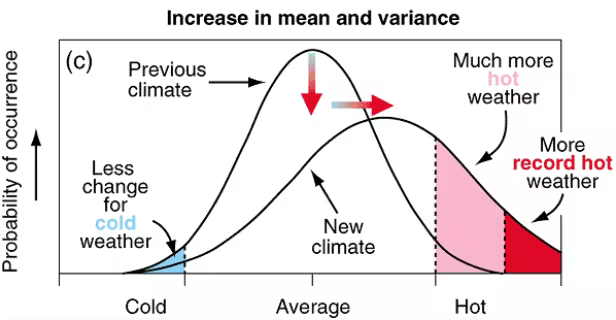
\includegraphics[width=0.6\linewidth]{fig/climate3} 

\end{figure}
\end{frame}

\begin{frame}[fragile]{Square root Transformation}
\phantomsection\label{square-root-transformation}
\begin{itemize}
\item
  \textbf{Square-root transformation}: This consists of taking the
  square root of each observation.
\item
  In R use: \textbf{sqrt(X)}
\end{itemize}

\begin{Shaded}
\begin{Highlighting}[]
\NormalTok{data }\OtherTok{\textless{}{-}} \FunctionTok{c}\NormalTok{(}\DecValTok{1}\NormalTok{, }\DecValTok{4}\NormalTok{, }\DecValTok{9}\NormalTok{, }\DecValTok{16}\NormalTok{, }\DecValTok{25}\NormalTok{, }\DecValTok{36}\NormalTok{, }\DecValTok{49}\NormalTok{, }\DecValTok{64}\NormalTok{, }\DecValTok{81}\NormalTok{, }\DecValTok{100}\NormalTok{)}
\CommentTok{\# Apply square{-}root transformation}
\NormalTok{sqrt\_data }\OtherTok{\textless{}{-}} \FunctionTok{sqrt}\NormalTok{(data)}
\CommentTok{\# Goodness of fit test}
\FunctionTok{shapiro.test}\NormalTok{(sqrt\_data)}
\end{Highlighting}
\end{Shaded}

\begin{verbatim}
## 
##  Shapiro-Wilk normality test
## 
## data:  sqrt_data
## W = 0.97016, p-value = 0.8924
\end{verbatim}
\end{frame}

\begin{frame}{Square root Transformation}
\phantomsection\label{square-root-transformation-1}
\begin{itemize}
\tightlist
\item
  If you apply a square root to a continuous variable that contains
  values negative values, decimals and values above 1, you are treating
  some numbers differently than others..

  \begin{itemize}
  \tightlist
  \item
    So a constant must be added to move the minimum value of the
    distribution to 1.
  \end{itemize}
\end{itemize}
\end{frame}

\begin{frame}[fragile]{Log Transformation}
\phantomsection\label{log-transformation}
\begin{itemize}
\item
  Many variables in biology have log-normal distributions.
\item
  In R use: \textbf{log(X)}
\end{itemize}

\begin{Shaded}
\begin{Highlighting}[]
\CommentTok{\# Sample data (e.g., positive values)}
\NormalTok{data }\OtherTok{\textless{}{-}} \FunctionTok{c}\NormalTok{(}\DecValTok{1}\NormalTok{, }\DecValTok{10}\NormalTok{, }\DecValTok{100}\NormalTok{, }\DecValTok{1000}\NormalTok{, }\DecValTok{10000}\NormalTok{, }\DecValTok{100000}\NormalTok{)}
\CommentTok{\# Apply log transformation (log base 10)}
\NormalTok{log\_data }\OtherTok{\textless{}{-}} \FunctionTok{log10}\NormalTok{(data)}
\CommentTok{\# Goodness of fit test}
\FunctionTok{shapiro.test}\NormalTok{(log\_data)}
\end{Highlighting}
\end{Shaded}

\begin{verbatim}
## 
##  Shapiro-Wilk normality test
## 
## data:  log_data
## W = 0.98189, p-value = 0.9606
\end{verbatim}
\end{frame}

\begin{frame}{Log Transformation}
\phantomsection\label{log-transformation-1}
\begin{itemize}
\tightlist
\item
  The logarithm of any negative number is undefined and log functions
  treat decimals differently than numbers \textgreater1.

  \begin{itemize}
  \tightlist
  \item
    SO a constant must be added to move the minimum value of the
    distribution to 1.
  \end{itemize}
\end{itemize}
\end{frame}

\begin{frame}[fragile]{Inverse transformation}
\phantomsection\label{inverse-transformation}
\begin{itemize}
\tightlist
\item
  \textbf{Inverse transformation}: This consists of taking the inverse
  (X-1) of a number.
\item
  In R use: 1/X or (X)\^{}-1
\end{itemize}

\begin{Shaded}
\begin{Highlighting}[]
\CommentTok{\# Sample data (e.g., positive values)}
\NormalTok{data }\OtherTok{\textless{}{-}} \FunctionTok{c}\NormalTok{(}\DecValTok{1}\NormalTok{, }\DecValTok{2}\NormalTok{, }\DecValTok{4}\NormalTok{, }\DecValTok{8}\NormalTok{, }\DecValTok{16}\NormalTok{, }\DecValTok{32}\NormalTok{, }\DecValTok{64}\NormalTok{)}
\CommentTok{\# Apply inverse transformation (reciprocal)}
\NormalTok{inverse\_data }\OtherTok{\textless{}{-}} \DecValTok{1} \SpecialCharTok{/}\NormalTok{ data}
\end{Highlighting}
\end{Shaded}

\begin{itemize}
\tightlist
\item
  Tends to make big numbers small and small numbers big a constant must
  be added to move the minimum value of the distribution to 1
\end{itemize}
\end{frame}

\begin{frame}{Reflecting Transformations}
\phantomsection\label{reflecting-transformations}
\begin{itemize}
\tightlist
\item
  Each of these transformations can be adjusted for negative skew by
  taking the reflection
\item
  To reflect a value, multiply data by -1, and then add a constant to
  bring the minimum value back above 1.0\\
\item
  For example:

  \begin{itemize}
  \tightlist
  \item
    Square root sqrt (X) becomes

    \begin{itemize}
    \tightlist
    \item
      sqrt ( {[}(X*-1)+c{]})
    \end{itemize}
  \item
    Log ln (X) becomes - ln ({[}X*-1{]} +c)
  \end{itemize}
\end{itemize}
\end{frame}

\begin{frame}{Rank Transform}
\phantomsection\label{rank-transform}
\end{frame}

\begin{frame}{Transformation Rules to Live By}
\phantomsection\label{transformation-rules-to-live-by}
\begin{itemize}
\item
  Transformations work by altering the relative distances between data
  points.
\item
  If done correctly, all data points remain in the same relative order
  as prior to transformation.
\item
  However, this might be undesirable if the original variables were
  meant to be substantively interpretable.
\item
  Therefore\ldots{}
\end{itemize}
\end{frame}

\begin{frame}{Transformation Rules to Live By}
\phantomsection\label{transformation-rules-to-live-by-1}
\begin{itemize}
\tightlist
\item
  Don't mess with your data unless you have to.
\end{itemize}

\begin{itemize}
\tightlist
\item
  Are there true outliers? Remove and retest.
\end{itemize}

\begin{itemize}
\tightlist
\item
  If you have to mess with it, make sure you know what you are doing.
  Try different transformations to see which is best.
\end{itemize}

\begin{itemize}
\tightlist
\item
  Include these details in your methods.
\end{itemize}

\begin{itemize}
\tightlist
\item
  Back transform to original units for reports of central tendency and
  variability.
\end{itemize}

\begin{itemize}
\tightlist
\item
  Sometimes transformations don't work, don't panic, you will just get
  to run \textbf{nonparametric tests}.
\end{itemize}
\end{frame}

\end{document}
